\documentclass[10pt]{article}
\usepackage[letterpaper,margin=.78in]{geometry}
\usepackage{amsmath,booktabs,array,graphicx,hyperref,xurl}
\hypersetup{hidelinks,pdftitle={S27-B: Tokenizer by Backend Interaction},pdfauthor={Research execution record}}
\graphicspath{{../figures/}}\setlength{\parskip}{4pt}
\title{S27-B: Tokenizer by Backend Interaction}
\author{Research execution record}\date{23 November 2026}
\begin{document}\maketitle
\section{Question and Frozen Execution}
Does the HStem-versus-Long-Patch accuracy difference depend on the selected backend? This experiment uses the S27 B design frozen before its execution, on top of S27-A commit \texttt{636da47}. Twelve new source-only fits replace the two MHA blocks by the already defined two-block positionwise residual TokenMLP; twelve original HStem/Long-Patch MHA checkpoints are reused. No source packet, seed, readout width or optimizer is selected from B target scores.

Each MLP block is $h'=\operatorname{LN}(h+W_2\operatorname{GELU}(W_1h))$, with width 128 and 16,704 parameters versus 16,768 for MHA. The full-model difference is 128 parameters. The 32-by-64 interface, input projection, position terms, pre-LN, final-LN, mean pooling and classifier remain unchanged. Corresponding surviving initial parameters and paired data/noise streams match; the two new heads share a fixed CPU initialization stream. Different nonlinear forms, token interactions, expressivity and computation remain; parameter matching does not isolate only attention.

The new fits use two folds, seeds 201/202/203, five legal source RXs, 8,000 train and 2,000 source-validation packets, 200 epochs, batch 64, AdamW, five warmup epochs/cosine schedule and AWGN 0--50dB. Only clean source RX-equal CE selects checkpoints. All twelve new checkpoint/config/history hashes are sealed and committed before any new Dev inference; both new arms are completed before target results are observed. C, IQ-only, ASK Strict-IB and further readout search remain unexecuted.
\section{All Four Cells and Primary Interaction}
\begin{center}\small\begin{tabular}{lrrrrrrr}\toprule
Cell&Params&Dev acc.&Fit SD&Macro-F1&Worst RX&Source acc.&Source CE\\\midrule
HS/MHA&133,690&97.335&0.552&97.326&93.667&98.175&0.05902\\
LP/MHA&138,346&94.500&1.831&94.423&88.333&96.358&0.10702\\
HS/MLP&133,562&96.448&1.204&96.391&86.450&97.875&0.07196\\
LP/MLP&138,218&93.402&0.824&93.305&83.933&94.725&0.14573\\
\bottomrule\end{tabular}\end{center}
Accuracy/F1 are percentages, fit SD is over six fold/seed means in pp, and worst RX is the minimum three-seed RX mean. Source validation has already participated in selection. HS denotes HStem; LP denotes the fixed freely learned long projection.
\begin{align*}
\Delta_M&=A_{HS,MHA}-A_{LP,MHA},\\
\Delta_P&=A_{HS,MLP}-A_{LP,MLP},\\
\Delta_{int}&=\Delta_M-\Delta_P.
\end{align*}
The complete-cohort tokenizer contrasts are $\Delta_M=+2.835$pp and $\Delta_P=+3.047$pp. The primary interaction is -0.212pp, conditional RX95\% interval [-0.845,0.600], with 2/6 positive paired interactions. Fold means are +0.247 and -0.670pp.
The registered positive rule is not met. A small difference or an interval containing zero does not prove equivalence or that attention is useless.
The unchanged rule requires mean at least .5pp, positive conditional lower bound, at least 5/6 positive fit interactions and positive means in both folds. Three seeds are first averaged within each of ten unique RXs; 10,000 RX bootstrap repetitions use seed 27028. Intervals omit new-seed, acquisition and architecture-selection uncertainty. Secondary contrasts are descriptive, without multiplicity-corrected confirmatory claims.
\begin{figure}[htbp]\centering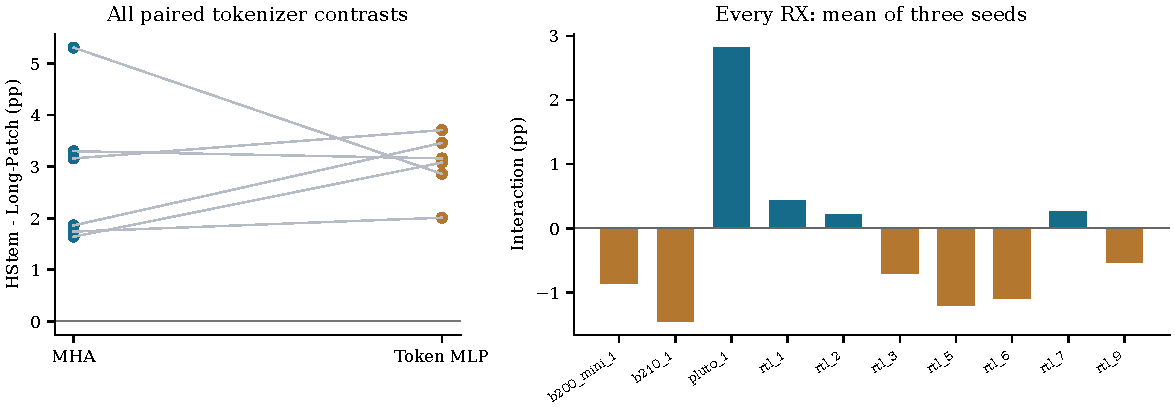
\includegraphics[width=.98\linewidth]{fig01_interaction.pdf}
\caption{Every paired tokenizer difference and every RX interaction. Negative and zero effects remain visible.}\end{figure}
\section{Source Learning, Historical Dev, and Scope}
Source interaction is -1.333pp, compared with -0.212pp on Dev. Source-minus-Dev interaction is -1.122pp. All six paired values are archived.
Both chosen backends preserve positive HStem-minus-LP differences in all six fit pairs and all ten RX means. This secondary observation does not meet the primary MHA-amplification criterion or establish equivalence. The HStem MHA-minus-MLP difference is +0.887pp; Pluto's +7.217pp contributes +0.722pp to the unchanged ten-RX mean. RTL5 and RTL6 favor MLP. No RX is removed from the primary estimate.
Source validation uses 40 selected packets/TX/RX and already selects checkpoints; Dev uses 200 and has a development history. Source/Dev differences do not replace a freshly fitted four-source/one-held-source study. Poor source learning by an MLP control also limits assigning its errors entirely to receiver transfer. A positive interaction cannot alone establish receiver-specific robustness.
\begin{figure}[htbp]\centering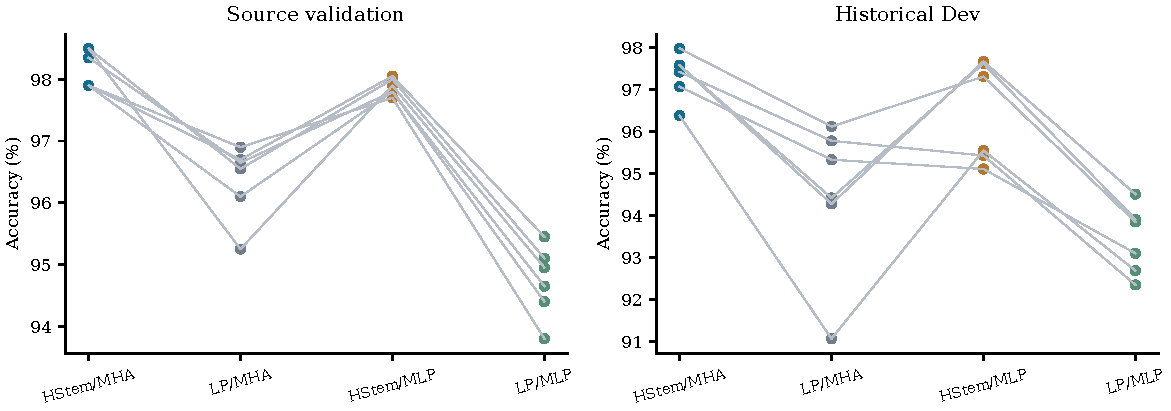
\includegraphics[width=.98\linewidth]{fig02_fourcells.pdf}
\caption{Complete source and Dev accuracies of all 24 frozen models; no weak fit is excluded.}\end{figure}
\clearpage
\section{Fixed-Layer Source Geometry}
All 24 models use the same 2,000 legal source-validation packets/fold. The taps are mean tokenizer output, mean after input projection/position/pre-LN and final classifier input, each 64D. Pooling precedes per-packet L2 normalization. Balanced 40-packet TX-by-RX cells use the original S25 between-TX scatter $B$, conditional RX scatter $D$, within-cell scatter $W$, $J_c=B/(D+10^{-12})$ and $J_w=B/(D+W+10^{-12})$ definitions. The table averages six per-fit statistics, not pooled features or a ratio of overall means. If any fit is invalid, its entire arm/layer aggregate is NA; no replacement normalization is chosen.
\begin{center}\small\begin{tabular}{llrrrrr}\toprule
Cell&Tap&$B$&$D$&$W$&$J_c$&$J_w$\\\midrule
HS/MHA & tokens & 0.0386 & 0.0030 & 0.0413 & 14.1252 & 0.9826\\
HS/MHA & pre\_backend & 0.0636 & 0.0018 & 0.0191 & 33.9828 & 3.1026\\
HS/MHA & final & 0.8172 & 0.0235 & 0.1275 & 35.5774 & 5.4487\\
LP/MHA & tokens & 0.0060 & 0.0006 & 0.0078 & 9.3358 & 0.4962\\
LP/MHA & pre\_backend & 0.0471 & 0.0015 & 0.0114 & 37.1227 & 3.8214\\
LP/MHA & final & 0.7905 & 0.0274 & 0.1450 & 29.1354 & 4.6030\\
HS/MLP & tokens & 0.2405 & 0.0060 & 0.0515 & 40.0871 & 4.2493\\
HS/MLP & pre\_backend & 0.2130 & 0.0041 & 0.0279 & 52.4286 & 6.7230\\
HS/MLP & final & 0.6861 & 0.0182 & 0.0822 & 37.8927 & 6.8439\\
LP/MLP & tokens & 0.0218 & 0.0037 & 0.0644 & 6.8954 & 0.3231\\
LP/MLP & pre\_backend & 0.1537 & 0.0040 & 0.0360 & 39.0842 & 3.9001\\
LP/MLP & final & 0.6623 & 0.0171 & 0.0974 & 39.0070 & 5.8609\\
\bottomrule\end{tabular}\end{center}
\begin{figure}[htbp]\centering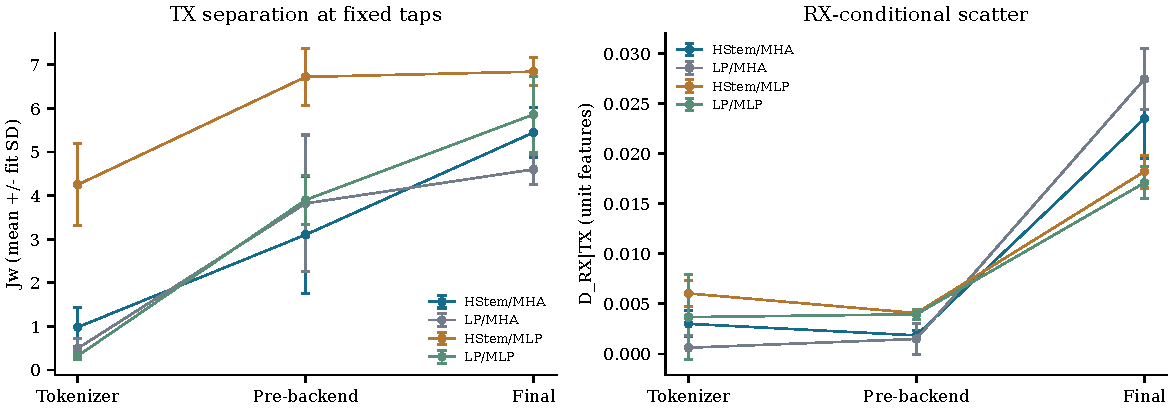
\includegraphics[width=.98\linewidth]{fig03_source_geometry.pdf}
\caption{All three fixed taps and all four cells. Error bars are fit SD. Mean 64D diagnostics do not summarize all information in the full token sequence.}\end{figure}
The models are trained end to end; changing the backend also changes the learned tokenizer. Thus these comparisons are descriptive representations of different trained systems, not causal information flow through a fixed representation. Source-selected geometry, scatter and ratios do not establish mutual information, receiver removal or RF hardware invariance. This source execution preserves the original FP32/TF32 flags and is not numerically pooled with old TF32-off diagnostics.

The complete table contains counterexamples to a single-geometry explanation. MHA's pre-backend $J_w$ is lower for HStem than LP. For both tokenizers, the MLP final-source $J_w$ is higher than MHA's, while Dev accuracy is lower. Under MLP, final conditional RX scatter is higher for HStem than LP despite HStem's accuracy advantage. These fixed diagnostics therefore do not monotonically rank Dev accuracy or show that HStem removes RX information at every layer. The mean 64D taps do not characterize all information in the full token sequence.
\clearpage
\section{Every New Fit and Same-Session Cost}
\begin{center}\small\begin{tabular}{lrrrrrrr}\toprule
Cell&Fold&Seed&Best ep.&Source CE&Source acc.&Dev acc.&Fit wall(s)\\\midrule
HS/MLP & 0 & 201 & 197 & 0.06594 & 97.900 & 95.550 & 1941.8\\
LP/MLP & 0 & 201 & 140 & 0.14479 & 94.950 & 92.690 & 2078.3\\
HS/MLP & 0 & 202 & 176 & 0.06256 & 98.000 & 95.110 & 1945.8\\
LP/MLP & 0 & 202 & 171 & 0.14165 & 95.100 & 93.100 & 2084.9\\
HS/MLP & 0 & 203 & 193 & 0.05596 & 98.050 & 95.430 & 1976.4\\
LP/MLP & 0 & 203 & 166 & 0.12103 & 95.450 & 92.350 & 2035.7\\
HS/MLP & 1 & 201 & 199 & 0.08490 & 97.800 & 97.670 & 1944.3\\
LP/MLP & 1 & 201 & 158 & 0.14358 & 94.650 & 94.510 & 2094.0\\
HS/MLP & 1 & 202 & 174 & 0.08050 & 97.700 & 97.310 & 1939.1\\
LP/MLP & 1 & 202 & 113 & 0.15816 & 93.800 & 93.850 & 2084.2\\
HS/MLP & 1 & 203 & 171 & 0.08192 & 97.800 & 97.620 & 1937.6\\
LP/MLP & 1 & 203 & 147 & 0.16515 & 94.400 & 93.910 & 1674.9\\
\bottomrule\end{tabular}\end{center}
Every new fit completes 200 epochs and 25,000 retained updates, without early stopping or target-driven reseeding. The twelve final trajectories total 300,000 scientific updates. After a user-requested pause, continuation was explicitly authorized on 23 November 2026. Three fits were complete; LP/MLP fold 0 seed 202 and HS/MLP fold 0 seed 203 resumed their saved complete-epoch states at epochs 180 and 3. Model, optimizer, RNG, registration and best-source-checkpoint consistency were verified before resuming; snapshot hashes and recovery receipts are archived. Work within an unsealed partial epoch may have been discarded, so 300,000 counts retained updates rather than all physical executions. Original and resumed controller logs are preserved separately. Summed fit wall times cover active execution segments, overlap under at most two CUDA jobs and are not exclusive GPU hours.
\begin{figure}[htbp]\centering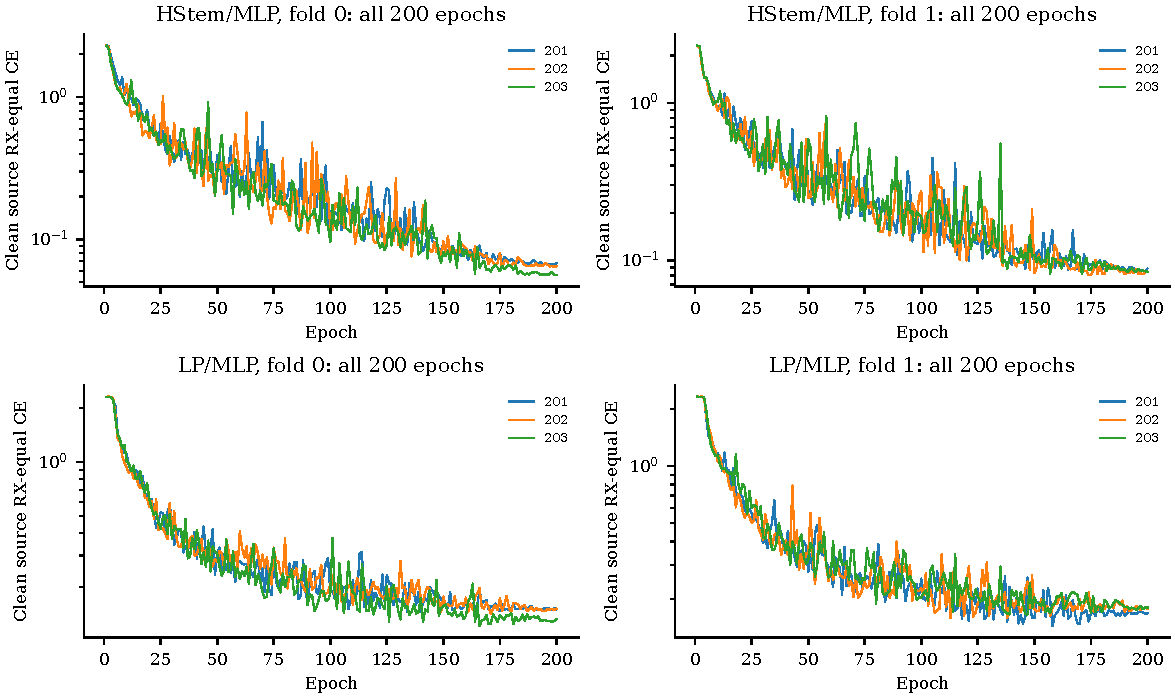
\includegraphics[width=.98\linewidth]{fig04_all_training.pdf}
\caption{All twelve source CE histories, all 200 epochs, no seed removed.}\end{figure}
\begin{center}\small\begin{tabular}{lrrr}\toprule
Cell&Partial MACs(M)&B1 p50(ms)&B128 p50(ms)\\\midrule
HS/MHA&95.028&2.464&17.652\\
LP/MHA&55.477&3.725&17.953\\
HS/MLP&94.766&5.307&18.109\\
LP/MLP&55.215&3.170&18.168\\
\bottomrule\end{tabular}\end{center}
This is one common GPU-resident IQ-to-logits timing session, batch 1/128, three warmups and 15 repetitions, original FP32 tensors with matmul TF32 off/cuDNN TF32 on. B128 is whole-batch latency. The latency includes FFT/frontend work and excludes host transfer. Partial MACs omit FFT and unsupported operations. Parameters, compute, latency and throughput are distinct axes; no old timing session is pooled here.
\section{Mechanism Judgment and Unexecuted C}
The registered positive interaction is not established. The current evidence supports a HStem-relative accuracy advantage under both selected backends; it does not support MHA amplification as an established explanation. An interval crossing zero does not demonstrate backend equivalence. Tokenwise MLPs also introduce different nonlinear forms, capacity and optimization paths. The source-geometry counterexamples prevent a single pooled scatter ratio from serving as a sufficient mechanism explanation.

If a receiver-specific gap claim is pursued, C remains necessary: B's five-source factorial training does not fit the predeclared four-source/one-held-source split. The fixed b210\_1/rtl\_5 pilot has only two held RX units and no population-RX guarantee. Current C, IQ-only and ASK Strict-IB fit counts are zero; no automatic expansion or new readout search follows these results. The existing innovation evidence matrix is updated without renaming old experiments. The formal TIFS manuscript is not rewritten in this stage.
\section{Integrity and Reproduction}
The engineering gate uses no RF data and separately records eight synthetic optimizer updates. It checks model shape/capacity, matching surviving initial states and MLP heads, finite gradients, exact optimizer/model/all-RNG recovery for both arms, forbidden data roles, batch 64/128 resources, bit-exact feature-hook forward results and four-cell interaction arithmetic. Unique-process JSON temporary files, bounded Windows rename retry and shared-delete progress reads preserve scientific update order.

Independent verification recomputes 240,000 Dev predictions, 48,000 source predictions and 72 geometry records, including balanced row/label identities, confusion matrices, accuracy/F1/CE, conditional interaction intervals, all 200-epoch minimum-source-CE histories, the original paired permutation and AWGN streams and historical model, configuration and history hashes. All 24 models and all RXs remain reported. No Confirm or old-blind packet, new target adaptation or fresh capture is introduced. Larger waveforms, checkpoints, resume states and per-packet predictions/features remain local; aggregate evidence, code and real logs are committed.

\href{https://github.com/hanCChan/crossatten/tree/exp/s27b-backend-interaction/27b-tokenizer-backend-interaction}{Repository evidence and Chinese mechanism report} accompanies this execution record. It supplies bounded architecture evidence, not submission-readiness or independent-generalization certification.
\end{document}
